\documentclass[12pt]{article}
\usepackage{t1enc}
\usepackage[utf8x]{inputenc}
%\usepackage[latin2]{inputenc} % ha a forrásszöveg iso8859-2 kódolású
\usepackage[magyar]{babel}
\usepackage{listings}
\usepackage[pdftex]{graphicx}
\usepackage{setspace}
\usepackage[nottoc, numbib]{tocbibind}
\usepackage[usenames, dvipsnames]{color}
\usepackage{parskip}
\usepackage[
    a4paper,
    top=2.5cm,
    bottom=2.5cm,
    inner=3.5cm,
    outer=2.5cm
]{geometry}
%\usepackage{epstopdf}
\usepackage{enumitem}
\usepackage[T1]{fontenc}
\usepackage{ae,aecompl}
\usepackage{amsmath}
\usepackage{amssymb}
\usepackage{amsthm}
\usepackage[a4paper]{geometry}
\usepackage{xcolor}
\usepackage{siunitx}
\usepackage{cleveref}
\usepackage[unicode, colorlinks=false, pdfborder={0 0 0}]{hyperref}
\usepackage{booktabs}
% bcs i am a fascist deep inside:
\usepackage{times} % Uncomment to use the Times New Roman font
\usepackage{microtype} % This should be the last one!
\usepackage{parskip}
\usepackage{pifont}
\usepackage{dsfont}
\def\DocTitle{Osztott rendszerek jegyzet}
\def\DocAuthor{Tóth Ákos}
\def\CurrentDate{2016}
\definecolor{clrNonExam}{gray}{0.3}
\linespread{1.3}
\onehalfspacing
\frenchspacing
\sloppy
\widowpenalty=30000
\clubpenalty=30000
\setlength{\parindent}{1.2em}
\setlength{\parskip}{1.0em}
\renewcommand{\baselinestretch}{1.0}
    \title{\DocTitle}
    \author{\DocAuthor}
    \date{\CurrentDate}
    \begin{document}
    \pagestyle{empty}
    \begin{titlepage}
        \begin{center}
            \Huge
            \textbf{\DocTitle}
            \normalsize
        \end{center}
        \vfill
        \begin{center}
            
\includegraphics[scale=1.0]{images/elte_cimer_szines.eps}
        \end{center}
        \vfill
        \begin{minipage}{1.0\linewidth}
            \begin{flushright}
                \textbf{\DocAuthor} \\
                Eötvös Loránd Tudományegyetem Informatikai Kar \\
                Programtervező Informatikus BSc C szakirány
            \end{flushright}
        \end{minipage}
        \vfill
        \begin{center}
            Budapest, \CurrentDate
        \end{center}
    \end{titlepage}
    \pagestyle{plain}
    \setcounter{page}{1}
    \section{Definíciók}
    \paragraph{Elosztott rendszer:}
    Önálló számítógépek olyan összessége, amely kezelői számára egyetlen
    koherens rendszernek tűnik.
    \paragraph{Nyitott elosztott rendszer:}
    A nyitott elosztott rendszer képes más nyitott rendszerek számára
    szolgáltatásokat nyújtani, és azok szolgáltatásait igénybe venni.
    Jellemző tulajdonságai, hogy jól definiált interface-el rendelkezik,
    valamilyen szintű hordozhatóság(\textit{portability}) és
    együttműködési (\textit{interoperability}) (más
    rendszerekkel), támogatása. 
    \section{Kérdések és válaszok}
    \subsection{Rövid kérdések}
    \paragraph{1. diasor}
    \begin{description}
        \item[Egy-egy mondattal jellemezz kétfajta (nem rokon jellegű)
            átlátszóságot.]
            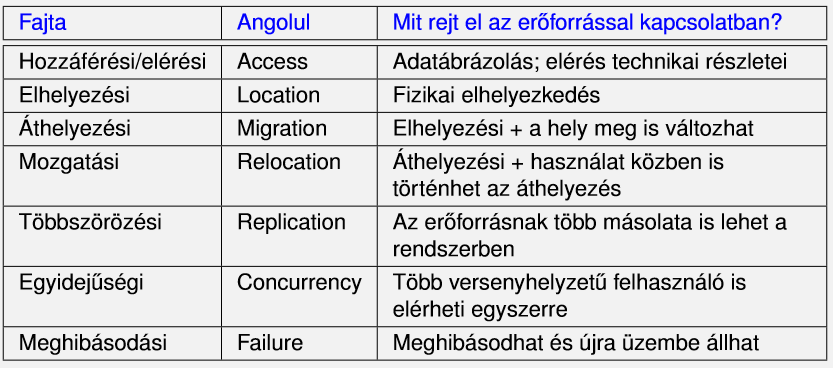
\includegraphics[scale=0.5]{images/P5.PNG}
        \item[Mi jellemzi a nyitott rendszereket?]
            \begin{itemize}
                \item jól definiált interface-kel rendelkeznek 
                \item Az alkalmazások hordozhatóságát minél inkább
                    támogatják(portability)
                \item könnyen elérhető a rendszerek
                    együttműködése(\textit{interoperability})
            \end{itemize}
        \item[Mi a nyitottság implementálásának főbb jellemzői?]
            \hfill
            \begin{itemize}
                \item Fontos, hogy a rendszer könnyen cserélhető részekből álljon
                \item Belső interface-k használata, nem egyetlen monolitikus
                    rendszer
                \item A rendszernek minél jobban paraméterezhetőnek kell lennie
            \end{itemize}
        \item[Egy-egy mondattal jellemezz kétfajta átméretezhetőséget.]
            \hfill
            \begin{itemize}
                \item Méret szerint: Több felhasznál és/vagy folyamat  (Könnyebben
                    kezelhető például erősebb szerverekkel!)
                \item Földrajzi: A rendszert nagyobb területen veszik igénybe:
                    egyetemen belüli felhasználás → világméretű felhasználóbázis
                \item Adminisztrációs: Biztonsági, karbantartási, együttműködési
                    kérdések merülnek fel, ha új adminisztrációs tartományok kerülnek
                    a rendszerbe
            \end{itemize}
        \item[Ismertess egy technikát, amelynek célja az átméretezhetőség
            megvalósítása.]
            \hfill
            \begin{itemize}
                \item A kommunikációs késleltetés elfedése
                    \begin{itemize}
                        \item Aszinkron kommunikáció használata
                        \item A beérkező választ külön kezelő dolgozza fel
                        \item Probléma, hogy nem minden alkalmazás ültethető át ilyen formában
                    \end{itemize}
                \item Elosztás 
                    \begin{itemize}
                        \item A számítások egy részét a kliensoldal végzi(Java
                            appletek)
                        \item Decentralizált elnevezési rendszerek(DNS)
                        \item Decentralizált információs rendszerek(WWW)
                    \end{itemize}
                \item Replikáció/cache-elés
                    \begin{itemize}
                        \item Replikált fájlszerverek és adatbázisok → inkonzisztencia veszélye → globális szinkronizáció szükséges(Rosszul skálázható!)
                        \item Tükrözött weboldalak
                        \item Fájlok cache-elés(böngészőkben, proxy szervereken)
                        \item Weboldalak cache-elés(a szerver- és kliensoldalon)
                    \end{itemize}
            \end{itemize}
        \item[Miben hasonlítanak és miben térnek el a cluster és a grid
            rendszerek?]
            \hfill
                    \begin{tabular}{c c c}
                        Clustera & | & Grid\\
                        \hline
                        &elosztott számítási rendszer&\\
                        lokális hálózat&&nagyméretű hálózat\\
                        központosított vezérlés&&átívelhet több szervezeti egységen\\
                        homogén számítógépek&&több, kevésbé egységes számítógép\\
                    \end{tabular}
        \item[Mi az ACID (Legalább két szempont részletezve, a másik kettőnek legalább a neve)?]
            \hfill
            Tranzakcióknál használt követelményrendszer:
            \begin{itemize}
                \item \textbf{Atomicity}: vagy a teljes tranzakció végbemegy vagy nem változik az adattár
                \item \textbf{Consistency}: A tranzakció konzisztens, ha érvényes állapotot állít elő. (csak a tranzakció lefutása után kell teljesülnie)
                \item \textbf{Isolation}: Egyszerre zajló tranzakciók nem zavarják egymást: olyan eredményt adnak, mintha egymás után sorban futottak volna le.
                \item \textbf{Durability}: Végrehajtás után az eredményt tartós adattárolóra mentjük, így a rendszer esetleges összeomlása után visszaállítható.
            \end{itemize}
        \item[Adj meg olyan feltételezést elosztott rendszerrel kapcsolatban, amellyel kényelmes élni, de a valóságban akadályokat gördíthet elénk.]
            \hfill
            \begin{itemize}
                \item a hálózat hibamentes
                \item a hálózat biztonságos
                \item a hálózat homogén
                \item a hálózati topológia nem változik
                \item a kommunikációnak nincsen időigénye
                \item a sávszélesség korlátlan
                \item a kommunikációnak nincsen költsége
                \item csak egy adminisztrátor van
            \end{itemize}
    \end{description}
    \paragraph{2. diasor}
    \begin{description}
    \item [Írd le az egyszerű kliens-szerver modellben a kommunikáció menetét.]
        \hfill
        \begin{enumerate}
            \item Kliens kérést küld a szervernek, majd várakozik a válaszra. 
            \item Szerver fogadja a kérés, válaszol.
            \item Kliens megkapja a választ, folytatja a működést. 
        \end{enumerate}
        \begin{center}
        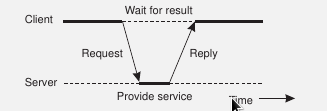
\includegraphics[scale=0.9]{images/CSCom.png}
        \end{center}
    \item[Milyen három rétegbe szokás osztani az alkalmazásokat?]
        \hfill
        \begin{itemize}
            \item Megjelenítés - felhasználó felületet alkotó komponensek (view)
            \item Üzleti logika - alkalmazás működését írja le konkrét adatok nélkül (controller)
            \item Perzisztencia - adatok tartós tárolása (model)
        \end{itemize}
    \item[Mi az "overlay"?]
        \hfill
        \begin{itemize}
            \item A gráfban szomszédos csúcsok a fizikai hálózaton lehetnek távol egymástól, a rendszer elfedi, hogy a köztük levő kommunikáció
                több gépet érintve történik.
            \item legtöbb P2P rendszer alapja
        \end{itemize}
    \item [Milyen az overlay peer-to-peer hálózatok felépítése?]
    \item  Nem találtam diában
    \item  Ismertess (nagyon) vázlatosan egy strukturált peer-to-peer rendszert.
    \item A csúcsokat valamilyen struktúra szerint overlay hálózatba
        szervezzük(pl\. logikai gyűrű),
        és a csúcsoktól az azonosítójuk alapján lehet szolgáltatásokat igénybe venni.
    \item Példa: elosztott hasítótábla Ebben a rendszerben kulcs-érték párokat tárolunk.
        Az adott értéket tároló csúcsot hatékonyan meg lehet keresni a kulcsa alapján, akármelyik csúcsra
        is érkezik be a kérés.
    \item Hogy működik a struktúrálatlan peer-to-peer pletykálás?
    \item selectPeer:
        - A részleges nézetből kiválaszt egy szomszédot.
    \item selectToSend: 
        - Az általa ismert szomszédok közül kiválaszt n darabot.
    \item selectToKeep:
        - A megkapott csúcsokat eltárolja lokálisan.
        - Eltávolítja a többszörösen szereplő csúcsokat.
        - A tárolt csúcsok számát m darabra csökkenti. Erre többfajta stratégia lehetséges.
    \item Hogyan működnek a struktúrálatlan peer-to-peer rendszerek?
    \item ezek a rendszerek igyekeznek véletlen gráf struktúrát fenntartani.
    \item Mindegyik csúcsnak csak részleges nézete van a gráfról 
    \item Minden P csúcs időközönként kiválaszt egy szomszédos Q csúcsot
        - P és Q információt cserél, valamint átküldik egymásnak az általuk ismert csúcsokat
    \item  Mi a superpeer? Egy-két mondattal jellemezz olyan rendszert, amelyben megtalálható.
    \item olyan kisszámú csúcs, amelyeknek külön feladata van
        - kereséshez index fenntartása
        - a hálózat állapotának felügyelete
        - csúcsok közötti kapcsolatok létrehozása
    \item Példa: nem találtam diában
    \item  Mi az interceptor?
    \item Távoli objektum elérése során a vezérlés szokásos menetébe avatkozik bele
        - pl. átalakíthatja más formátumra a kérést
    \item Jellemzően az architektúra rétegei közé illeszthető.
    \item  Milyen az önszervező rendszerek általános architektúrája?
    \item elvárható tulajdonságok
        - önkonfiguráló
        - önkezelő
        - öngyógyító
        - ön optimalizáló
        - ön*
    \item Mi az az edge server?
    \item az adatokat tároló szerver
    \item a kliensekhez minél közelebb van elhelyezve
    \item ahol egy nagyobb hálózat az Internetre csatlakozik
    \item Mi az a  Content Delivery Network?
    \item a tartalom szolgáltatás hatékonyságát növelik és költségét csökkentik.
    \item Adj módszert arra, hogyan válasszuk meg, melyik szerverek tároljanak egy adott fájlt
    \item visszacsatolásos modell
        - mérik, hogy a rendszer mennyire tér el a kívánt tulajdonságoktól, és szükség szerint változtatnak a
        beállításokon. ⇒ Például Globule
    \item Globule (CDN)
        - tartalmakat költségmodell alapján helyezi el
        - A központi szerver elemzi, hogy mi történt volna, ha P oldalt az S edge szerver tárolta volna.
        > A számításokat különböző stratégiákra végzi el, végül a legjobbat választja ki.
        3. diasor
    \item  Mi a kontextusváltás?
    \item A másik folyamatnak/szálnak történő  vezérlésátadás, illetve a megfelelő kontextusok cseréje. Így egy
        processzor több folyamatot/szálat is végre tud hajtani.
    \item  Milyen két fő megközelítés létezik a virtualizációra? Az egyik rövid jellemzésével.
    \item Process VM
        - a virtuális program közönséges programként fut ⇒ bytecode-ot hajt végre
        - példa : JVM , CLR
    \item VM Monitor
        - Hardver teljes körű virtualizációja ⇒ bármely operációs rendszer futtatására alkalmas
        - pl VirtualBox
    \item  Mi a szuperszerver?
    \item Olyan szerver, amelyik több porton figyeli a bejövő kapcsolatokat, és amikor új kérés érkezik, új folyamatot/szálat indít
        annak kezelésére. 
    \item  Mi a iteratív és konkurens szerver?
    \item iteratív  ⇒ egyszerre csak egy kapcsolatot tud kezelni
    \item konkurens ⇒ párhuzamosan több kapcsolatot is tud kezelni
    \item  Mi jellemzi az állapotteljes szervereket?
    \item Állapotot tart számon a klienstől
        - Megjegyzi, melyik fájlokat használta a kliens, és ezeket előre megtudja nyitni legközelebb
        - Megjegyzi, milyen adatokat töltött le a kliens, és frissítéseket küldhet neki
    \item  Mi a kódmigráció?
    \item olyan kommunikáció, amely során nem csak adatokat küldünk át
    \item  Nevezz meg legalább kétfajta feladatot, amely során kódmigráció történik, és részletezd az egyiket.
    \item Client-Server
        - a szokásos kliens-szerver kommunikáció, nincsen kódmigráció
    \item Remote Evaluation 
        - a kliens feltölti a kódot, és a szerveren futtatja
    \item Code on Demand 
        - a kliens letölti a kódot a szerverről, és helyben futtatja
    \item Mobile Agent 
        - a mobil ágens feltölti a kódját és az állapotát, és a szerveren folytatja a futását
    \item  Mik az objektum komponensek?
    \item Kódszegmens  ⇒ a programkódot tartalmazza
    \item Adatszegmens ⇒ a futó program állapotát tartalmazza
    \item Végrehajtási ⇒ szegmens: a futtató szál környezetét tartalmazza
    \item  Mi a gyenge mobilitás?
    \item a kód és az adatszegmens mozgatása (⇒ a kód újraindul)
        - Viszonylag egyszerű megtenni ha a kód hordozható
        - irány szerint
        > feltöltés(push,ship)
        > letöltés(pull, fetch)
    \item  Mi az erős mobilitás?
    \item A komponens végrehajtása szegmenssel együtt költözik
        - migráció ⇒ az objektum átköltözik egyik gépről másikra
        - klónozás ⇒ egy másolat kerül a másik gépre, mindkét gépen ugyanonnan folytatódik a futás
        4. diasor
    \item  Mi az ISO/OSI modell alsó három rétegének feladata?
    \item Fizikai réteg
        - a bitek átvitelének fizikai részei írja lefutása
    \item Adatkapcsolati réteg
        - az üzenetet keretekre tagolja
        - a hibajavítás és a hálózat terhelésének korlátozása
    \item Hálózati réteg
        - a hálózat távoli gépei között közvetít csomagokat útválasztás (routing) segítségével
    \item  Mi a szállítási réteg két fő protokollja, és ezeknek mik a főbb jellemzői?
    \item TCP ⇒ kapcsolatalapú, megbízható, sorrendhelyes átvitelének
    \item UDP ⇒ nem (teljesen) megbízható, általában kis üzenetek (datagram) átvitele	
    \item  Mi a köztes réteg?
    \item A köztes rétegbe (middleware) olyan szolgáltatásokat és protokollokat szokás sorolni, amelyek sokfajta alkalmazáshoz lehetnek hasznosak.
    \item  Mi jellemzi az időleges, szinkron kommunikációt?
    \item A kommunikációs rendszer elveti az üzenetet, ha az nem kézbesíthető.
    \item  Mi jellemzi a megtartó, aszinkron kommunikációt?
    \item A kommunikációs rendszer hajlandó huzamosan tárolni az üzenetet.
    \item  Milyen lépésekből áll az RPC hívás iránya?
        ⇒ A kliensfolyamat lokálisan meghívja a klienscsonkot
        ⇒ Az becsomagolja az eljárás azonosítóját és paramétereit, meghívja az OS-t.
        ⇒ Az átküldi az üzenetet a távoli OS-nek.
        ⇒ Az átadja az üzenetet a szervercsonknak.
        ⇒ Az kicsomagolja a paramétereket, átadja a szervernek.
        ⇒ A szerver lokálisan meghívja az eljárást, megkapja a visszatérési értéket.
        ⇒ Ennek visszaküldése a klienshez hasonlóan zajlik, fordított irányban.
    \item  Mit tud az RPC paraméter átadásról?
    \item kliens és szervergépen eltérhet az adatábrázolás ⇒ szerializálás szükséges
        - rögzíteni kell a paraméterek kódolását
        - A két csonknak fordítania kell a közös formátumról a gépeik formátumára
    \item Érték–eredmény szerinti paraméter átadási szemantika
    \item  Hogyan kezelhetőek a hivatkozások RPC hívás során?
    \item Távoli hivatkozás bevezetésével növelhető az elérési átlátszóságot
        - A távoli adat egységesen érhető el
        - A távoli hivatkozásokat át lehet paraméterként adni
        ebben nem vagyok biztos
    \item  Milyen lépésekből áll a socket kommunikáció? (Sorrenddel.)
    \item létrejön a socket
    \item csatlakozik a szerverhez( ⇒ a szerver fogadja a csatlakozást)
    \item a socket ír a szerverre ( ⇒ szerver fogadja majd válaszol)
    \item a socket fogadja a választ
    \item az előző két lépés tetszőleges számban ismétlődik
    \item a socket zárja a kapcsolatot
    \item  Adatátviteli módok folyamatos média esetén
    \item aszinkron
        - nem ad megkötést hogy mikor kell átvinni az adatot
    \item szinkron
        - az egyes csomagoknak egy bizonyos idő alatt kell a célba érniük
    \item izokron 
        - alsó és felső korlátot is ad a csomagok átvitelére
    \item  Mi a folyam? (Fontosabb jellemzőkkel.)
    \item adatfolyam
        - izokron kommunikációt támogató kommunikációs forma
    \item egyirányú
    \item legtöbbször egy forrástól(source) egy vagy több nyelő(sink) felé(gyakran közvetlenül csatlakozva hardverre)
    \item egyszerű folyam
        - egyfajta adatot továbbító
    \item összetett folyam
        - többfajta adatot továbbít
    \item  Miben tér el az anti-entrópia és a pletykálás alapú járványalgoritmus? (Előnyökkel, hátrányokkal.)
    \item Anti-entrópia
        - Minden szerver rendszeresen kiválaszt egy másikat
        - kicserélik egymás között a változásokat.
    \item Pletykálás (gossiping)
        - Az újonnan frissült (megfertőzött) szerver elküldi a frissítést néhány szomszédjának (megfertőzi őket).
    \item  Mi az a QoS?
    \item Quality of Service 
        - a folyamokkal kapcsolatban vázolt követelmények
    \item példa
        - a folyam átvitelének sebessége
        - a folyam megindításának legnagyobb késleltetése
        - stb...
    \item Biztosítása
        - differenciált szolgáltatás architektúra
        > hálózat router-i kategorizálják az áthaladó forgalmat 
        ⇒ egyes csomagfajta elsőbbséget élvez
        - remegés csökkentése
        > a router-k pufferelhetik az adatokat
        5. diasor
    \item  Mi a broadcasting?
    \item kihirdetjük az azonosítót a hálózaton ⇒ az egyed visszaküldi a jelenlegi címét
        - lokális hálózatokon túl nem skálázódik
        - a hálózaton minden gépnek figyelni kell a beérkező kérésre 
    \item  Mi a továbbító mutató?
    \item amikor az egyed elköltözik , egy mutató marad utána az új helyre
        - a kliens elől rejtve van
        - a megtalált cím visszaküldhető ⇒ további feloldások gyorsabbak
    \item  Mi a Chord elosztott hasítótábla?
    \item elosztott hasított táblát készítünk
        - csúcsok tárolnak egyedeket
        - N csúcsú gyűrű overlay szerkezetbe van szervezve
    \item minden csúcshoz véletlenszerű azonosító(m bit)
        - mindegyik entitáshoz kulcs(m bit)
    \item a :k kulcsú egyed felelőse az :id azonosítójú csúcs
        - k <= id és nincs köztük másik csúcs
        - jelölés
        > felelős csúcs a kulcs rákövetkezője
        > jel: succ(k)
    \item  Mit tartalmaz a Chord adatábrázolás egy finger table-je?
    \item minden p csúcs tárol FTp "finger table" -t m bejegyzéssel
        - FTp[i = succ(p\item2\^(i-)
            - bináris jellegű keresés ⇒ minden lépés felezi a keresési tartományt
            > 2\^(m-, 2\^(m-,\ldots,1
        \item  Mi az a HLS?
        \item Hierarchical Location Service
        \item A hálózatokat osszuk tartományokra
            - tartozzon minden tartományhoz egy katalógus
        \item építsünk hierarchiát a katalógusokból
        \item  Mik a katalógus csúcsok?
        \item az E egyed címe egy levélben található
        \item gyökértől az E levélig vezető úton minden belső csúcsban van egy mutató a következő gyerekre
        \item a gyökér minden út kiindulópontja
            - minden egyedről van információja
        \item  Jellemezd három szempont szerint, hogyan különbözik a DNS névtér három szintje.
        \item globális szint   ⇒ gyökér és felső csúcsok. A szervezetek közösen kezelik
        \item szervezeti szint ⇒ egy egy szervezet által kezelt csúcsok szintje
        \item kezelői szint    ⇒ egy adott szervezeten belül kezelt csúcsok
            szempont      |globális     | szervezeti | kezelői
            --------------\item-------------\item------------\item--------------------
            méret         | világméretű | vállalati  | vállalati alegység
            csúcsok száma | kevés       |sok         |rendkívül sok
            keresés ideje | mp.         |ezredmp.    | azonnal
        \item  Hogyan működik az iteratív névfeloldás?
        \item gyökér névszerverek egyikétől indítjuk
        \item a névnek csak egy komponensét oldjuk fel
            - a megszólított névszerver az ehhez tartozó névszerver címét küldi vissza
        \item  Hogyan működik a rekurzív névfeloldás?
        \item a névszerverek egymás között kommunikálva oldják fel a nevet
            - a kliens oldali név feloldóhoz rögtön a válasz érkezik
        \item  Mit mondhatunk a névfeloldás átméretezhetőségéről?
        \item problémák 
            >> sok kérés rövid idő alatt ⇒ globális szint szerverei nagy terhelés kapnának
            >> földrajzi távolságokat is figyelembe kell venni
            >> egy adott csúcsot egy adott névszerver szolgál ki , földrajzilag oda kell csatlakozni
        \item csúcsok adatai sok névszerveren
            - felső két szinten alig változik a gráf
            - legtöbb csúcs adatairól másolatok készíthetők több névszerverre
        \item keresett adat az entitás címe
            - névszerverek nem alkalmasak mozgó entitások címeinek kezelésére >>  mert azok költözésével változna a gráf
        \item  Mi az X.500?
        \item A katalógus szolgáltatásokban az attribútumokra érvényes megkötések egyfajta szabványa
        \item LDAP protokollon szokás elérni 
        \item Az elnevezési rendszer fastruktúrájú
            - élei attribútum-érték párokkal címzettek
            - Az egyedekre az útjuk jellemzői vonatkoznak, és további párokat is tartalmazhatnak.
            6. diasor
        \item  Hogyan működik a Cristian-algoritmus?
        \item mindegyik gép egy központi időszervertől kéri le a pontos időt (Network Time Protocol)	
            - Nem a megkapott időre kell állítani az órát: bele kell számítani, hogy 
            a szerver kezelte a kérést és a válasznak vissza kellett érkeznie a hálózaton keresztül
        \item  Hogyan működik a Berkeley-algoritmus?
        \item Itt nem feltétlenül a pontos idő beállítása a cél, csak az, hogy minden gép ideje azonos legyen.
            - álagot von minden gép idejéből
            ⇒ majd mindenkit értesít, hogy a saját óráját mennyivel kell átállítania
            - Az idő egyik gépnél sem folyhat visszafelé: ha vissza kellene állítani valamelyik órát,
            akkor ehelyett a számontartott idő mérését lelassítja a gép mindaddig, amíg a kívánt idő be nem áll.
        \item  Hogyan működik az előbb történt (happened - before) reláció?
        \item Ha ugyanabban a folyamatban az a esemény korábban következett be beseménynél, akkor a -> b
        \item Ha a esemény egy üzenet küldése, és b esemény annak fogadása, akkor a -> b
        \item A reláció tranzitív:  ha a -> b és b -> c, akkor a -> c
        \item  Az idő és az előbb történt reláció kapcsolata?
        \item Minden e eseményhez időbélyeget rendelünk, ami egy egész szám (Jelölése:  C(e)) és megköveteljük az alábbi tulajdonságokat:
            - Ha a -> b egy folyamat két eseményre, akkor C(a) < C(b)
            - Ha a esemény egy üzenet küldése és b esemény annak fogadása, akkor C(a) < C(b)
        \item  Mi a Lamport-féle időbélyeg?
        \item Minden Pi folyamat saját Ci számlálót tart nyilván az alábbiak szerint: 
            - Pi minden eseménye eggyel növeli a számlálót
            - Az elküldött m üzenetre ráírjuk az időbélyeget: ts(m) = Cj
            - Ha az m üzenet beérkezik Pj folyamathoz, ott a számláló új értéke Cj = max{Cj, ts(m)}\item1 lesz így az idő nem folyik visszafelé
            - Pi és Pj időbélyegei közül tekintsük a Pi-belit elsőnek, ha i < j
        \item  Mi az időbélyeg-vektor?
        \item A Pi most már az összes másik folyamat idejét is számon tartja egy VCi[1...n tömbben,
                ahol VCi[j azoknak a Pj folyamatban bekövetkezett eseményeknek a száma, amelyekről Pi tud
                \item Az m üzenet elküldése során Pi megnöveli eggyel  VCi[i értékét, és a teljes Vi időbélyeg-vektort ráírja az üzenetre
                    \item Amikor az m üzenet megérkezik a Pj folyamatkozhoz, amelyekre a ts(m) időbélyeg van írva, két dolog történik:
                        - VC,[k := max{VCj[k, ts(m)[k}
                                    - VCj[j megnő eggyel, vagyis az üzenet fogadása is egy eseménynek számítani
                                    \item  Pontosan sorbarendezett csoportcímzés definíciója?
                                    \item Az időbélyeg-vektorokkal megvalósítható a pontosan sorbarendezett csoportcímzés: csak akkor kézbesítjük az üzeneteket,
                                        ha már mindegyik előzményüket kézbesítettük.
                                    \item  Kölcsönös kizárás feladata?
                                    \item Több folyamat egyszerre szeretne hozzáférni egy adott erőforráshoz. Ezt egyszerre csak egynek engehetjük meg közülük,
                                        különben az erőforrás helytelen állapotba kerülhet
                                    \item Megoldásfajták: 
                                        - Központi szerver
                                        - Peer-to-peer rendszereken alapuló teljesen elosztott megoldás
                                        - Teljesen elosztott megoldás ált. gráfszerkezetre
                                        - Teljesen elosztott megoldás gyűrűben
                                    \item  Ismertesd a központosított kölcsönös kizárási algoritmust.
                                    \item Tegyük fel, hogy az erőforrás n-szeresen többszörözött, és minden replikátumhoz tartozik egy azt kezelő koordinátor.
                                        Az erőforráshoz való hozzáférésről többségi szavazás dönt: legalább m koordinátor engedése szükséges, ahol m > n/2.
                                        Feltesszük, hogy egy esetleges összeomlás után a koordinátor hamar felépül - azonban a kiadott engedélyeket elfelejti.
                                    \item  Elosztott kölcsönös kizárás működési elve?
                                    \item Ismét többszörözött az erőforrás, amikor a kliens hozzá szeretne férni, kérést küld mindegyik koordinátornak. Választ akkor kap, ha
                                        - a koordinátor nem igényli az erőforrást, vagy
                                        - a koordinátor is igényli az erőforrást, de kisebb az időbélyegei
                                        - különben a koordinátor nem válaszol
                                    \item  Ismertesd a zsetongyűrű alapú kölcsönös kizárási algoritmust.
                                    \item A folyamatokat logikai gyűrűbe szervezzük. A gyűrűben egy zsetont küldünk körbe, amelyik folyamat birtokolja,
                                        az férhet hozzá az erőforráshoz
                                    \item  Csúcsok globális pozícionálása. Meg szeretnénk becsülni a csócsok közötti kommunikációs költségeket. Erre többek között azért van szükség, hogy hatákonyan
                                        tudjuk megválasztani, melyik gépekre helyezzünk replikátumokat az adatainkból.
                                    \item Ábrázolás: A csúcsokat egy többdimenziós geometriai térben ábrázoljuk, ahol a P és Q csúcsok közötti kommunkiációs költséget a csócsok távolsága jelöli.
                                    \item  Zsarnok-algoritmus
                                        A folyamatoknak sorszámot adunk. A legnagyobb sorszámű folyamatot szeretnénk vezetőnek választani.
                                        - Bármelyik folyamat kezdeményezhet vezetőválasztást. Mindegyik folymatnak elküld egy választási üzenetet
                                        - Ha Pnagyobb üzenetet kap Pkisebb-től, visszaküld neki egy olan üzenetet, amellyel kiveszi Pkisebb-et a választásból
                                        - Ha P megadott időn belül nem kap letiltó üzenetet, ő lesz a vezető. Erről mindegyik másik folyamatot értesíti egy üzenettel.
                                    \item  Vezetőválasztás gyűrűben
                                        Logikai gyűrűnk vagy, és a folyamatoknak vannak sorszámai. A legnagyobb sorszámú folyamatot szeretnénk vezetőnek választani.
                                    \item Bármelyik folyamat kezdeményezhet vezetőválasztást: elindít egy üzenetet gyűrűn körbe, amelyekre mindenki ráírja a sorszámát.
                                        Ha egy folyamat összeomlott, az kimarad
                                    \item Amikor az üzenet visszajut a kezdeményezőhöz, minden aktív folyamat sorszáma szerepel rajta. Ezek közül a legnagyobb lesz a vezető.
                                    \item Nem okozhat problémát, ha több folyamat is egyszerre kezdeményez választást	
                                    \item  Superpeer-választás:
                                    \item A többi csúcs alacsony késleltetéssel éri el őket
                                    \item Egyenletesen vannak elosztva a hálózaton
                                    \item A csúcsok megadott hányadát választjuk superpeer-nek
                                    \item Egy superpeer korlátozott számú peer-t szolgál ki
                                        7. diasor
                                    \item  Mi az a Conit?
                                    \item egy olyan adategység amelyre közös feltételrendszer vonatkozik(consisteny unit)
                                        - amennyiben megtehetjük hogy konzisztenciafeltételeket az adatok minnél szűkebb körére írjuk fel
                                    \item  Mi az a soros konzisztencia?
                                    \item elvárjuk hogy a végeredmény olyan legyen , mintha az összes folyamat összes művelete
                                        egy meghatározott sorrendben történt volna meg
                                        - megőrizve bármely adott folyamat saját műveleteinek sorrendjét
                                    \item  Mi az okozati konzisztencia?
                                    \item A potenciálisan okozatilag összefüggő műveleteket kell mindegyik folyamatnak azonos sorrendben látnia.
                                        - A konkurens írásokat különböző folyamatok különböző sorrendben láthatják.
                                    \item  Milyen megközelítése lehetnek a szinkronizációs változóknak?
                                    \item Egy rendszerszintű S változó használata
                                        - S egy elérése után garantált, hogy a korábbi elérései előtti írások megtörténtek
                                    \item Változók  igénylése/feloldása ⇒ kritikus területek
                                        - több rendszerszintű szinkronizációs változó használata
                                        - minden adatelemhez külön változó
                                    \item  Adj módszert arra, hogyan válasszuk meg sok klienst kiszolgáló szerverek helyeit (közel) optimálisan nagy hálózatban.
                                    \item válasszuk meg ugy a szerverek helyét, a kliensektől vett átlagtávolsága minimális legyen.
                                        >> egzakt kiszámítása költséges, heurisztika szükséges
                                    \item a K legnagyobb renszerben helyezzünk el egy-egy szervert, mindig a rendszeren belül, leginkább közpoti helyre
                                        >>  szintén magas számítási költség
                                    \item Keressük meg a K legsűrűbb részt, és oda helyezzünk szervereket(d-dimenziós ábrázolás esetén, távolság = késleltetés)
                                        >> számítási költsége alacsonyabb	
                                    \item  Milyen lehetősége vannak tartalom replikálására?
                                    \item tartós másolat
                                        - a folyamat mindig rendlkezik másolattal (origin server)
                                    \item szerver által kezdményezett másolat
                                        - replikátum kihelyezése egy szerverre, amikor az igényli az adatot
                                    \item kliens által kezdeményezett másolat
                                        - kliensoldali gyorsítótár
                                    \item  Replikátum frissítése során milyen adatokat küldhetünk át a szerverek között?
                                    \item Kizárólag frissítésről szóló értesítés / érvénytelenítés
                                    \item Passzív replikáció
                                        - adatok átvitele egyik másolatról a másikra
                                    \item Aktív replikáció
                                        - frissítés művelet átvitele
                                    \item  Mi a haszonbérlet?	
                                    \item a szerver ígéretet tesz a kliensnek, hogy elküldi neki a frissítéseket míg a haszonbérlet aktív
                                    \item  Mi a rugalmas haszonbérlet?
                                    \item rendszer állapotától függhet a haszonbérlet időtartama
                                        - kor szerint 
                                        > minnél réggebben változott az objektum, annál valószínűbb hogy az is marad 
                                        ⇒ hosszabb lejárat adható
                                        - igénylés gyakorisága szerint
                                        > minél gyakrabban igényli a kliens az objektumot, annál hosszabb időtartamokra kap haszonbérletet rá
                                        - terhelés szerint
                                        - minél nagyobb a szerver terhelése, annál rövidebb haszonbérleteket ad ki 
                                    \item  Hogyan működik az elsődleges másolaton alapuló protokoll távoli írással?	
                                    \item Példa
                                        - a másolatok gyakran egy lokális hálózatra kerülnek
                                        - kapcsolat nélküli munka, időnként szinkronizál a rendszerrel	
                                    \item  Hogyan működik a testületalapú protokoll? Milyen feltételek kikötésével lehet garantálni a helyességet?
                                    \item Többszörözött írás
                                        - az írási műveletet több szerveren hajtjuk végre.
                                    \item Testület (quorum): 
                                        - egy művelet végrehajtása előtt meghatározott számú szervertől kell engedélyt kérni.
                                        8. diasor
                                    \item  Komponens helyessége
                                    \item elérhetőség       ⇒ a komponens reagál a megkeresésre
                                    \item megbízhatóság     ⇒ a komponens biztosítja a szolgáltatást
                                    \item biztonságosság    ⇒ a komponens ritkán romlik el
                                    \item karbantarthatóság ⇒ az elromlott komponens könnyen javítható
                                    \item  mi a hibajelenség?
                                    \item a komponens nem tőle a tőle elvártaknak megfelelően üzemel
                                    \item  mi a hiba?
                                    \item olyan rendszerállapot ami hibajelenséghez vezethet
                                    \item  mi a hibaok?
                                    \item a hiba (feltételezett) oka
                                    \item  Hibákkal kapcsolatos tennivalók
                                    \item Megelőzés
                                    \item Hibatűrés
                                        - a komponens legyen képes elfedni a hibát
                                    \item Mérséklés
                                        - lehet mérsékelni a hibák kitejedését, számát , súlyosságát
                                    \item Előrejelzés
                                        - előre becsülhető lehet a hibák száma, következményei
                                    \item  Milyen lehetséges hibaokok vannak?
                                    \item Összeomlás
                                        - a komponens leáll de előtte helyesen működik
                                        >> Probléma: Nem különbötethető meg hogy összeomlott vagy csak lassú 
                                    \item kiesés
                                        - a komponens nem válaszol
                                    \item időzítési hiba
                                        - a komponens helyes választ küld , de túl lassan
                                    \item válaszhiba
                                        - a komponens hibás választ küld
                                        > értékhiba
                                        > állapotátmeneti hiba
                                    \item váratlan hiba
                                        - véletlenszerű válaszok , véletlenszerű időzítéssel
                                    \item  Milyen csoportak vannak folyamatok esetén?
                                    \item egyenlő csoport
                                        - jó hibatűrés
                                        > csoport tagjai között közvetlen az információ csere
                                        - nehéz implementáció
                                        > a vezérlés teljesen elosztott
                                    \item hierarchikus csoport
                                        - két fél csak a koordinátoron keresztül kommunikál
                                        >> Rossz a hibatűrése és a skálázhatósága
                                        - könnyű implementálni
                                    \item  Csoport tagság kezelése
                                    \item csoportkezelő
                                        - egy koordinátor kezeli a csoportot
                                        >> rosszul skálázódik
                                    \item csoportkezelők csoportja
                                        - a csoportkezelő nem egyetlen szerver
                                        > ezt is kezelni kell , viszont ezek a szerverek elég stabilak
                                    \item csoportkezelő nélkül
                                        - a belépő / kilépő folyamat minden csoporttagnak üzenetet küld
                                    \item  Mit kell tudni a csoportkban történő hibaelfedésről?
                                    \item k-hibatűrő csoport
                                        - olyan csoport amely képes elfedni k tag egyszerre történő meghibásodását
                                    \item folyamatok
                                        - a folyamatok azonos ütemben lépnek-e
                                    \item késleltetések
                                        - a kommunikációs késleltetésekre van-e felső korlát
                                    \item rendezettség
                                        - az üzeneteket a feladás sorrendjében kézbesítik-e
                                    \item átvitel
                                        - egyenként (unicast)
                                        - többcíműen (multicast)
                                    \item lehetséges feltételrendszerek a közös végredményhez 
                                        - Ha az ütemezés szinkron és a késleltetés korlátozott.
                                        - Ha az üzeneteket sorrendtartó módon, többcíműen továbbítjuk.
                                        - Ha az ütemezés szinkron és a kommunikáció sorrendtartó.
                                    \item  Hogyan észlelhetők a hibák?
                                    \item időtúllépés észlelése
                                        - időkorlát megadása alkalmazásfüggő >> nehéz
                                        - folyamat / hálózat hiba nem megkülönböztethető
                                        - hibákról értesíteni kell a rendszer többi részét
                                        > pletykálás
                                        > az észlelő komponens is hibaállapotba megy
                                    \item  Milyen hibajelenségek lehetnek RPC esetén?
                                    \item  kliens nem találja  szervert
                                        ⇒ egyszerű kijelezni a kliensnél
                                    \item a kliens kérése elveszett
                                        ⇒ a kliens újraküldi a kérést
                                    \item a szerver összeomlott
                                        >> nehéz kezelni >> a kliens nem tudja mennyire lett feldolgozva a kérés
                                    \item elveszett a szerver válasza
                                        >> nehéz felismerni >> kliens szemszögéből szerver összeomláshoz hasonlít
                                    \item összeomlik a kliens
                                        >> szerver feleslegesen foglal erőforrásokat >> árva feladatok
                                        ⇒ feladatokra időkorlát
                                        ⇒ szerver leállítja/visszagörgeti az árva feladatokat
                                    \item  Hogyan működik a 2PC?
                                    \item two-phase commit
                                        - koordinátor K 
                                        > számítást kezdeményező kliens
                                        - résztvevő R
                                    \item működés
                                        - 1/K
                                        > megkérdez mindenkit, enged e commitolni(vote-request)
                                        - 1/R
                                        > igen(vote-commit) vagy nem(vote-abort) válasz ⇒ utóbbinál eldobja a kiszámított értéket
                                        - 2/K
                                        > ha minden válasz igen ⇒ global-commit üzenet
                                        > különben ⇒ global-abort
                                        - 2/R
                                        > végrehajtja a globális utasítást
                                    \item blokkolódhat
                                        - ha a koordinátor és legalább egy résztvevő összeomlik
                                        - szinte sosem fordul elő gyakorlatban
                                    \item  Hogyan működik a 3PC?
                                    \item működés
                                        - 1/K
                                        > vote-request
                                        - 1/R
                                        > vote-commit vagy vote-abort
                                        - 2/K
                                        > van vote-abort ⇒ mindenkinek global-abort 
                                        > minden vote-commit ⇒ mindenkinek prepare-commit
                                        - 2/R
                                        > prepare -commit esetén ⇒ ready-commit válasz
                                        > különben leáll 
                                        - 3/K
                                        > összegyüjti a prepare-commit üzeneteket ⇒ mindenkinek global-commit
                                        - 3/R
                                        > fogadja global-commit-ot , elmenti az adatokat
                                    \item nem blokkolódhat
                                        - koordinátor és résztvevők legfeljebb 1 távol
                                        - ha minden aktív résztvevő READY ⇒ a kiesett érsztvevő nem lehet COMMIT fázisban
                                    \item  mik lehetnek a felépülés irányai?
                                    \item előrehaladó felépülés
                                        - új állapotba hozzuk a rendszert ahonnan működhet
                                    \item visszatérő felépülés
                                        - egy korábbi érvényes állapotra térünk vissza
                                        > ehhez ellenőrzőpontokat veszünk fel
                                    \item  Mi a konzisztens metszet?
                                    \item olyan ellenőrzőpont-gyűjtemény, amelyben minden beérkezett üzenethez a küldési esemény is el van tárolva
                                    \item  Mi a felépülési vonal?
                                    \item a lehető legkésőbb készült konzisztens metszet
                                    \item  Mi az a dominóeffektus?
                                    \item vissza akarjuk kresni a legutolsó konzisztens metszetet
                                        ⇒ minden folyamatban visszatérés egy korábbi ellenőrzőponthoz
                                        >> elküldetlen üzenetek további üzeneteket tesznek nem elküldötté
                                    \item hátha ez is kellde nem biztos (87-
                                        jelölések üzenetek naplózására?
                                    \item HDR[m 
                                            - m az üzenet fejléce 
                                        \item COPY[m
                                                - azok a folyamatok amelekhez HDR[m megérkezett, de még nem tárolták
                                                \item DEP[m
                                                        - azok a folyamatok, amelyekhez megérkezett HDR[m' 
                                                            > ahol m' okozatilag függ m től
                                                        \item  Mikor stabil egy üzenet?
                                                        \item ha a fejléce már biztosan nem veszeht el
                                                        \item  Mi a pesszimista naplózóprotokoll?
                                                        \item ha m nem stabil akkor megköveteljük hogy legfeljebb egy folyamat függjön tőle
                                                            > |DEP[m| <= 1
                                                            \item  Mi az optimista naplózóprotokoll?
                                                            \item tfh C hibás folyamatok halmaza
                                                            \item nem stabil m üzenetekre igaz hogy COPY[m rész C -nek
                                                                    > ekkor egy idő után teljesüljön DEP[m része C -nek  is 
                                                                        10. diasor
                                                                    \item  Távoli elosztott objektumok
                                                                    \item Objektum: műveleteket és adatokat zár egységbe (enkapszuláció)
                                                                    \item A műveleteket metódusok implementálják, ezeket interfészekbe csoportosítjuk
                                                                    \item Az objektumokat csak az interfészükön keresztül érhetik el a kliensek
                                                                    \item Az objektumokat objektumszerverek tárolják
                                                                    \item A kliensoldali helyettes (proxy) megvalósítja az interfészt
                                                                    \item A szerveroldalon a váz kezeli a beérkező kéréseket
                                                                    \item  Objektumok létrehozása
                                                                    \item ideje alpján:
                                                                        - Fordítási időben létrejövő objektumok: A helyettest és a vázat a fordítóprogram készíti el,
                                                                        összeszerkeszti a kliens és a szerver kódjával
                                                                        - Futási időben létrejövő objektumok: Tetszőleges nyelven valósítható meg, de objektumadapterre van
                                                                        szükség a szerveroldalon a használatához
                                                                    \item élettartam alapján:
                                                                        - Átmeneti (tranziens) objektum: Élettartama csak addig tart, amíg be van töltve a szerverbe. 
                                                                        Ha a szerver kilép, az objektum is megsemmisül
                                                                        - Tartós (perzisztens) objektum: Az objektum állapotát és kódját lemezre írjuk, így a szerver kilépése után
                                                                        is megmarad.
                                                                    \item  Enterprise Java Beans (EJB)
                                                                    \item Az objektumokat alkalmazásszerverek tárolják (pl. GlassFish), amelyek lehetővé teszik az objektumok
                                                                        különböző módokon való elérését
                                                                    \item Fajtái:
                                                                        - Statless session bean: Tranziens objektum, egyszer hívják meg, miután elvégezte a feladatát megszűnik.
                                                                        Példa: egy SQL lekérdezés végrehajtása és az eredmény átadása a kliensnek
                                                                        - Stateful session bean: Tranziens objektum, de a klienssel egy munkameneten keresztül tartja a kapcsolatot,
                                                                        ezalatt állapotot is tart fenn. Példa: bevásárlókosár
                                                                        - Entity bean: Perzisztens, állapottal rendelkező objektum, amely több munkamenetet is ki tud szolgálni
                                                                        Példa: olyan objektum, amely az utolsó néhány kapcsolódó kliensről tárol adatokat
                                                                        - Message-driven bean: Különböző fajta üzenetekre reagálni képes objektum. A publish/subscribe kommunikációs
                                                                        modell szerint működik
                                                                    \item  Globe elosztott objektumok
                                                                    \item A Globe rendszerekben az objektumok fizikailag több gépen helyezkednek el: elosztott közös objektum(distributed shared object, DSO).
                                                                    \item  Objektumszerverek
                                                                    \item A rendszer részei a kiszolgálók, a vázak és az adapterek
                                                                    \item A kiszolgálót, amely az objektum működését biztosítja, több paradigma szerint lehet implementálni:
                                                                        - Függvények gyűjteménye, amelyik adatbázistáblákat, rekordokat stb.
                                                                        manipulálasznak
                                                                        - Osztályok
                                                                    \item A váz szerveroldali hálózati kapcsolatokat kezeli:
                                                                        - Kicsomagolja a beérkező kéréseket, lokálisan meghívja az objektumot, becsomagolja és visszaküldi a választ
                                                                        - Az interfész specifikációja alapján hozzák létre
                                                                    \item Az objektumadapter feladata az objektumok egy csoportjának kezelése:
                                                                        - Elsőként fogadja a kéréseket és azonosítja a releváns kiszolgálót
                                                                        - Aktivációs házirend (policy) szerint aktiválja  a megfelelő vázat
                                                                        - Az adapter generálja az objektumhivatkozásokat 
                                                                    \item  Távoli metódushívás (RMI)
                                                                    \item Tegyük fel, hogy a helyttes és a váz rendelkezésre áll a kliensnél/szervernél
                                                                        - A kliens meghívja helyettest
                                                                        - A helyettes becsomagolja a hívás adatait és elküldi a szervernek
                                                                        - A szerver biztosítja, hogy a hivatkozott objektum aktív
                                                                        - Az objektum váza kicsomagoja a kérést és a metódus meghívodik
                                                                        - Ha paraméterként objektumhivatkozást kaptunk, ezt szintén távoli metódushívással ér el a szerver,
                                                                        ebben a szerver kliensként vesz részt
                                                                        - A választ hasonló úton küldjük vissza, a helyettes kicsomagolja és visszatér vele a klienshez
                                                                    \item  RMI paraméterátadás
                                                                    \item Hivatkozás szerinti paraméterátadás:
                                                                        - A szerver egyszerűen távoli, metódushívással éri el az objektumot
                                                                        - Ha már nincsen szüksége rá, megszünteti a csatolást (unbind)
                                                                    \item Érték szerinti paraméterátadás: 
                                                                        - Szerializálni kell az objektumot:
                                                                        - Az állapotát
                                                                        - A metódusait, vagy hivatkozását olyan helyre, ahol alérhető az implementációjuk
                                                                        - Amikor a szerver kicsomagolja az objektumot, ezzel másolat készül az eredetiról
                                                                        - Ez az automatikus másolódás többféle problémát okoz Példa: néha túl átlátszó
                                                                    \item  Konzisztencia 
                                                                    \item Az objektumok a belépő konzisztencia megvalósításának természetesen adódó eszközei
                                                                        - Az adatok egységbe vannak zárva, és szinkronizációs változóval védjük őket
                                                                        - A szinkronizációs változókat soros konzisztencia szerint érjük el
                                                                        - Az adatokat kezelő műveletek összessége pont az objektum interfésze lesz
                                                                    \item  Milyen probléma merül fel, ha többszörözött objektumok hívják
                                                                        egymást, és hogyan lehet megoldani?  
                                                                    \item Replikált objektumok: Nemcsak a kéréseknek kell sorrendben beérkezniük a replikátumokhoz, a vonatkozó szálak ütemezésének
                                                                        determinisztikusnak kell lennie
                                                                    \item Replikált hívások:
                                                                        - Aktív replikáció: Ha a replikált objektum hívás során maga is meghív más objektumot, az a kérést többszörözve kapná meg
                                                                        Mo.: mind a szerver-, mint a kliensobjektumon válasszunk koordinátort és csak a koordinátorok küldhessenek kéréseket és válaszokat
                                                                        11. diasor
                                                                    \item  Hogyan működik a Network File System (NFS)?
                                                                    \item Network File System
                                                                        - elosztott fájlok távoli elérése
                                                                        - alkamazások a hely Virtual File System réteget érik el(távoli elérés átlátszósága)
                                                                    \item működés
                                                                        System call layer ⇒ VFS ⇒ RPC client stub ⇒ RPC server stub ⇒ VFS 
                                                                    \item  Cluster alapú fájlrendszerek.  
                                                                    \item kliens - szerver megközelítés nem elég jó 
                                                                    \item fájlok felbontésa csíkokra , részek párhuzamos elérése
                                                                        - rendszer gyorsítása
                                                                        - biztonságossá tétele
                                                                    \item Példa: Google File System
                                                                        - központ csak azt tárolja , melyik szerver melyik részek felelőse
                                                                        - elsődleges másolaton alapuló protokoll
                                                                        > központot nem terheli
                                                                    \item  Milyen vonatkozásban jelenik meg az RPC fájlrendszerekben?
                                                                    \item Egy lehetőség távoli fájlrendszerek megvalósítására, ha távoli eljáráshívások segítségével végezzük a fájlműveleteket.
                                                                    \item Példa
                                                                        - NFSv4 ⇒ támogatja műveletek összekombinálását egy hívásba
                                                                    \item  Mit lehet mondani a fájlmegosztás szemantikájáról?  
                                                                    \item Ha egyszerre több kliens is hozzáférhet egy fájlhoz, a konkurens írási és olvasási műveletek lehetséges végrehajtási sorrendjeit és a kijöhető eredmények
                                                                    \item Fajtái
                                                                        - Megváltoztathatatlan fájlok
                                                                        > fájlok tartalmát nem lehet módosítani létrehozás után
                                                                        > ritkán alkalmazható
                                                                        - UNIX szemantika
                                                                        > olvasási eredmények mindig a legutolsó írási művelet eredményét adják
                                                                        - Tranzakciós szemantika
                                                                        > a rendszer minden fájlra külön biztosít tranzakciókat
                                                                        - Munkamenet szemantika
                                                                        > ha a kliens megnyitja a fájl , amíg vissza nem írja az írási és olvasási műveletek csak saját maga számára látszanak
                                                                    \item  Mit lehet tudni a Coda fájlrendszerről 
                                                                    \item kliensek cache-elhetik a fájlokat
                                                                        >> replikált fájlok esetén költséges a kérések sorrendjének kikényszerítése
                                                                        >> ha összeomlik egy kliens, hosszu idő után jöhet a következő
                                                                    \item munkamenetei tranzakciós szemantikát valósítanak meg
                                                                        - A megnyitott fájl tartalma átmásolódik a kliensre
                                                                        > ha más módosítja a fájlt, arról a kliens értesítést kap.
                                                                        - Ha a kliens csak olvas akkor folytathatja a működését 
                                                                        > úgy tekintjük, hogy a tranzakció, amelyet végez, már korábban lezárult.	
                                                                    \item  Mi a kliensoldali gyorsítótárazás célja?
                                                                    \item főleg a teljesítmény növelés
                                                                    \item szerver kiiértesítő őket ha megvonják ezt a jogot
                                                                    \item  Mi a szerveroldali gyorsítótárazás célja?
                                                                    \item hibatűrés biztosítása
                                                                    \item  Hogyan növelhető P2P rendszerek rendelkezésre állása?
                                                                    \item decentralizált fájlrendszer
                                                                        - probléma lehet ha túl gyorsan változik a tagság >> kiléphet akár egy fájlt tartalmazó összes csúcs
                                                                        ⇒ replikálhatjuk fájljainkat (aránya r\_rep)
                                                                        ⇒(erasure coding) F fájlt bontsuk m részre , majd minden szerverre
                                                                        tegyünk n részt ( n > m) (aráyna r\_ec = n/m) 
                                                                        > változékony rendszerekben(r\_ec < r\_rep)
                                                                        12. diasor
                                                                    \item  Elosztott webalapú rendszerek
                                                                    \item A WWW (World Wide Web) olyan szerverek összessége, amelyek HTTP protokollon keresztül különféle tartalmakat szolgálnak ki
                                                                        A dokumentumokat hiperhivatkozások kapcsolják össze
                                                                        - Sok dokumentum szövegalapú: szövegfálj, HTML, XML
                                                                        - Egyéb fajták: képek, audio, videó, dokumentum
                                                                        - A tartalmak lehetnek a kliensoldalon végrehajthatóak (Javascript)
                                                                    \item  Webszolgáltatások.
                                                                    \item Felmerült az is, hogy felhasználó < - > weboldal interakció mellett az oldalak is igénybe vehetnek szolgáltatásokat más
                                                                        oldalakról -- > fontos, hogy a szolgáltatások szabványosak legyenek
                                                                    \item  Webszerverek.
                                                                    \item A szerver szerkezetét a tartalmak kiszolgálásának menete szabja meg. A szerverekbe beépülő modulok telepíthetők,
                                                                        amelyek a kiszolgálás egyes fázisaiban aktivizálódnak
                                                                    \item  Szerverfürtök    
                                                                    \item A teljesítmény és a rendelkezésre állás növelésének érdekében a szerverek sokszor többszörözve vannak.
                                                                        A kapcsolattartó szűk keresztmetszetté válhat, ennek elkerülésére több lehetőség van:
                                                                        - TCP átadás: Valamilyen metrika alapján kiválasztunk egy szervert és a kliens kiszolgálását az a szerver folytatja
                                                                        - Taralomérzékeny kéréselosztás: A HTTP kérés tartalmát is figyelmebe vesszük a szerver kiválasztásánál. Ez megnöveli
                                                                        a kpacsolattartó terhelését, de sok előnye van: segítségével hatékonyabban lehet a szerveroldali cache-elés, és lehetnek
                                                                        bizonyos feladatokra dedikált szervereink
                                                                    \item  Webhelyettes
                                                                        A kimenő kapcsolatok kezelésére webhelyetteseket (web proxy) telepíthetünk. Ezek cache-elik a kiszolgált tartalmakat,
                                                                        csak akkor fordulnak a szerverekhez, ha sem náluk, sem a többi helyettesnél nincsen meg a kért tartalom
                                                                    \item  Replikáció webkiszolgálókban
                                                                    \item A replikáció célja a teljesítmény növelése. A rendszer paraméterei változóak lehetnek, ezeket célszerű önszabályozással beállítani
                                                                    \item  Szerveroldali replikáció.
                                                                    \item A tartalomkézbestő hálózatok (CDN) nagy teljesítményű és rendelkezésre állású elosztott rendszerek, amelyeknek célja
                                                                        dokumentumok hatékony kiszolgálása
                                                                    \item  Replikáció webalkalmazásokban
                                                                    \item Ha a CDN tárolt adataiban változás következik be, ez először az eredetszerveren jelenik meg. A változásokat el kell juttatni
                                                                        a CDN szerverekhez, ennek a célszerű módja a rendszer jellegétől függ
                                                                        - Teljes replikáció: sok olvasás, kevés írás, öszetett lekérdezések
                                                                        - Részleges replikáció: sok olv., kevés írás, egyszerű lekérdezések
                                                                        - Tartalom szerinti gyorsítótárazás: Az adatbázist az edge szerver módosított, a lekérdezésekhez illeszkedő alakban
                                                                        tárolja helyben, és feliratkozik a szerveren a frissítésekre. Jól működik intervallumokra vonakozó, összetett lekérdezésekre
                                                                        - Eredmények gyorsítótárazása: Az edge szerver a korábbi lekérdezések eredményeit tárolja el. Jól működik egyszerű
                                                                        lekérdezések, amelyek egyedi adatokra vonatkoznak
                                                                    \item Ha az írások számaránya megnő, akkor a replikáció akár ronthatja is a rendszer teljesítményét 
                                                                        \color{clrNonExam}
                                                                    \item Hogyan történik a nyitottság implementálása?
                                                                        \begin{itemize}
                                                                            \item Fontos, hogy a rendszer könnyen cserélhető részekből álljon
                                                                            \item Belső interfészek használata, nem egyetlen monolitikus rendszer
                                                                            \item A rendszerknek minél jobban paraméterezhetőnek kell lennie.
                                                                            \item Egyetlen komponens megváltoztatása/cseréje lehetőleg minél
                                                                                kevésbé hasson a rendszer más részeire.
                                                                        \end{itemize}
                                                                    \item Melyek az elosztott rendszer céljai?
                                                                        \begin{itemize}
                                                                            \item Távoli erőforrások elérhetővé tétele
                                                                            \item Átlátszóság (distribution transparency)
                                                                            \item Nyitottság (openness)
                                                                            \item Skálázhatóság (scalability)
                                                                        \end{itemize}
                                                                    \item  Mely szempontok alapján épül fel egy elosztott rendszer?
                                                                        \begin{itemize}
                                                                            \item Független számítógépek
                                                                            \item Egyetlen rendszer ⇒ köztes réteg (middleware)
                                                                        \end{itemize}
                                                                    \item
                                                                        Melyek az elosztott rendszerek fajtái:
                                                                        \begin{itemize}
                                                                            \item
                                                                                számítási
                                                                            \item
                                                                                információs
                                                                            \item
                                                                                beágyazott/átható
                                                                        \end{itemize}
                                                                        \begin{center}
                                                                        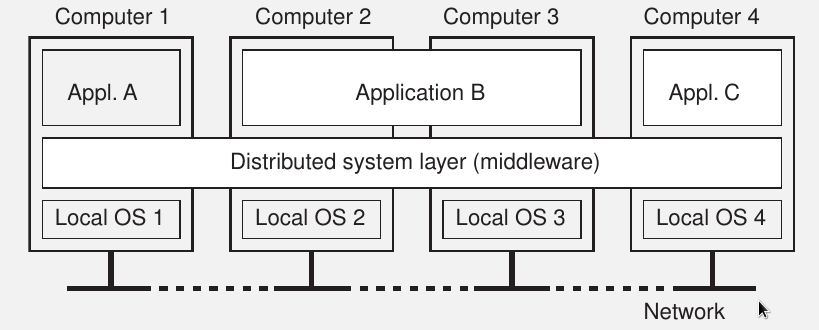
\includegraphics[scale=0.5]{images/ElosztottRendszer.png}
                                                                    \end{center}
                                                                \end{description}
                                                                \subsection{Kifejtős kérdések}
                                                                \begin{description}
                                                                    \item  Milyen átfogó célokat fogalmazhatunk meg elosztott rendszerekkel kapcsolatban? Milyen fő szempontok tartoznak a célokhoz? Mennyire megvalósíthatóak a célok, milyen akadályok merülnek fel?
                                                                        Célok:
                                                                    \item Távoli erőforrások elérhetővé tétele
                                                                    \item Átlátszóság
                                                                    \item Nyitottság
                                                                    \item Skálázhatóság
                                                                        Átlátszóság: (! a törekvés általában túl erős)
                                                                    \item A felhasználók különböző kontinenseken is lehetnek 
                                                                    \item Meghibásodások elfedése lehetetlen
                                                                        - Összeomlott a szerver vagy lassan válaszol? 
                                                                        - Összeomlás előtt feldolgoztat-e az adatot
                                                                    \item nagyméretű átlátszóság ⇒ hatékonyság romlása
                                                                        - webes gyorsítótárak tökéletesen frissen tartása
                                                                        - minden azonnal lemezre írása
                                                                        Nyitottság: 
                                                                    \item a rendszer legyen képes más nyitott rendszerekkel együtt dolgozni
                                                                        - jól definiált interface-k
                                                                        - alkalmazások hordozhatóságának támogatása
                                                                        - könnyen eléhető a rendszerek együttműködése
                                                                    \item legyen alkalmazható heterogén(különböző) környezetben
                                                                        - hardvereken
                                                                        - platformokon
                                                                        - programozási nyelveken
                                                                    \item implementálása
                                                                        - A rendszer könnyen cserélhető részekből álljon
                                                                        - Belső interface-k használata, nem egyetlen monolitikus rendszer
                                                                        - a rendszernek minnél jobban paraméterezhetőnek kell lennie
                                                                        - egyetlen komponens megváltoztatása/cseréje minnél kevésbé hasson a a rendszer más részeire
                                                                    \item probléma
                                                                        - kozisztencia
                                                                        - adatok megbízhatósága
                                                                        Skálázhatóság:
                                                                    \item jellege
                                                                        - méret szerint   ⇒ több felhasznál és/vagy folyamat  (! könnyebben kezelhető például erősebb szerverekkel )
                                                                        - földrajzi       ⇒ a rendszert nagyobb területen veszik igénybe
                                                                        - adminisztrációs ⇒ biztonsági, karbantartási, együttműködési kérdések
                                                                    \item megvalósítások és problémák 
                                                                        - kommunikációs késletetés elfedése 
                                                                        > aszinkron kommunikáció >> nem minden alkalmazás ültethető át ilyen megközelítésre
                                                                        - elosztás 
                                                                        > a számítások egy részét a kliensoldal végzi
                                                                        > decentralizált elnevezési/információs rendszerek
                                                                        - replikáció/cache
                                                                        > replikált fájlszerverek és adatbázisok >> inkozisztencia veszélye >> globális szinkronizáció szükséges(! rosszul skálázható)
                                                                        > tükrözött weboldalak
                                                                        > fájlok/weboldalak cache-elése
                                                                    \item  Milyen főbb fajtái vannak az elosztott rendszereknek? Milyen feladatok megoldására alkalmasak, milyen szerveződésűek?
                                                                        Elosztott számítási rendszerek(⇒ számítások végzése nagy teljesítménnyel)
                                                                    \item Cluster
                                                                        - lokális hálózatra kapcsolt számítógépek összessége 
                                                                        - homogén (ugyanaz az os, hardveresen nem vagy alig térnek el)
                                                                        - a vezérlés központosítva van általában egyetlen gépre
                                                                    \item Grid
                                                                        - több gép, kevésbé egységesek
                                                                        - átívelhet több szervezeti egységen 
                                                                        - nagyméretű hálózatokra terjedhet ki 
                                                                    \item Cloud(többrétegű architectúra)
                                                                        - Hardver
                                                                        - Infrastruktúra(⇒ virtuális hardvert tesz elérhetővé)
                                                                        - Platform
                                                                        - Alkalmazás
                                                                        Elosztott információs rendszerek(⇒  adatok kezelése, már meglévő ilyen rendszerek elérése)
                                                                    \item A tranzakció adatok összességén végzett művelet az alábbi tulajdonságokkal
                                                                        - atomicity
                                                                        - consistency
                                                                        - isolation
                                                                        - durability
                                                                    \item A tranzakciókat esetenként több szerver végzi ezeket egy TP monitor vezérli 
                                                                        >> Probléma :  A TP monitor nem választja el az alkalmazásokat az adatbázisoktól,  az alkalmazásoknak egymással is kommunikálniuk kell.
                                                                        Elosztott átható rendszerek(⇒ sok kicsi mobil elemből áll)
                                                                    \item A környzet változhat ⇒ a rendszernek ezt követnie kell
                                                                    \item Ad hoc szerveződés ⇒ komponensek különbözően használhatók ⇒ könnyen konifurálhatóság szükséges
                                                                    \item Megosztott szolgáltatások ⇒ változékobny rendszer az adatoknak könnyen kell áramolni ⇒ egyszerű szerkezetű elemek
                                                                    \item  Mik a szálak és mik a folyamatok? Hogyan viszonyulnak egymáshoz? Mikor melyiket érdemes alkalmazni? Hogyan jelennek meg kliens-szerver kapcsolatokban?	
                                                                        Szál:
                                                                    \item a processor egyfajta szoftveres megfelelője, minimális kontextussal
                                                                    \item a kontextus elmenthető, és később visszatölthető továbbfuttatáshoz 
                                                                        Folyamat:
                                                                    \item egy vagy több szálat összefogó nagyobb egységen
                                                                    \item egy folyamat szálai közös memóritaterületen dolgoznak
                                                                    \item különböző folyamatok nem látják egymás memóriaterületét
                                                                        Kontextus:
                                                                    \item Szál
                                                                        - nem sokkal bővebb a processorkontextusnál
                                                                        - szálak közötti váltáshoz nem kell os támogatása
                                                                    \item Folyamat
                                                                        - tartalom jórészét az MMU kezeli
                                                                        - folyamatok létrehozása / törlése / váltása költséges 
                                                                        Szálak elhelyezkedése:
                                                                    \item Folyamaton belül(szálkönyvtár)
                                                                        - előny
                                                                        > minden műveletet egyetlen folyamaton belül kezelünk, ez hatékony
                                                                        - hátrány
                                                                        > minden művelet a gazdafolyamattól >> ha a kernel blokkolja a szálat, a folyamat is blokkolódik
                                                                        > ha a kernel nem látja a szálakat, hogy közvetit neki szignálokat?
                                                                    \item Folyamaton kívül(kernelszintű szálak)
                                                                        - előny
                                                                        > A szálak blokkolása nem okoz problémát
                                                                        > A szignálokat a kernel a megfelelő szálhoz tudja irányítani
                                                                        - hátrány
                                                                        > Mivel minden művelet a kernelt érinti, ez a hatékonyság rovására megy
                                                                    \item Solaris szálakat
                                                                        - könnyűsúlyú folyamat ⇒ kernelszintű szálak , amelyek felhasználói szintű szálkezelőket futtatnak
                                                                        Kliens oldalon:
                                                                    \item Példa: többszáló webkliens (⇒ hálózati késé elfedése)
                                                                        - A böngésző letöltött egy oldalt, ami több másik tartalomra hivatkozik.
                                                                        - Mindegyik tartalmat külön szálon tölti le, amíg a HTTP kéréseket kiszolgálják, ezek blokkolódnak.
                                                                        - Amikor egy-egy fájl megérkezik, a blokkolás megszűnik, és a böngésző megjeleníti a tartalmat.
                                                                        Szerver oldalon:
                                                                    \item Cél: hatékonyság növelése
                                                                        - Szálak olcsóbbak mint a folyamatok
                                                                        - többprocesszoros rendszerek kapacitását csak többszálú szerverek képesek kihasználni
                                                                        - hálózat késleltetését lehet elfedni
                                                                    \item Cél: program szerkezetének javítása
                                                                        - A program jobban kezelhető lehet, ha sok egyszerű, blokkoló hívást alkalmaz, mint más szerkezet esetén. (>> némi teljesítményvesztés)
                                                                        - kisebbek és könnyebben érthetőek 
                                                                    \item  Hasonlítsd össze távoli szolgáltatások igénybe vételének különböző modelljeit: kliens-szerver, RPC, RMI, MOM.
                                                                        Kliens-szerver
                                                                    \item általános jellemzők
                                                                        - jellemzően szinkron kommunikáció
                                                                        - kliensnek és szervernek egyidőben kell aktívnak lennie
                                                                        - a kliens blokkolódik amíg a válasz meg nem érkezik
                                                                        - a szerver csak a kliensek fogadásával és a kérések kiszolgálásával foglalkozik
                                                                    \item szinkron kommunikáció hátrányai
                                                                        - a kliens nem dolgozik amíg a válaszra vár
                                                                        - a hibákat rögtön kezelni kell vagy feltartjuk a klienst
                                                                        - bizonyos feladatokhoz(levelezés) nem jól illeszkedik
                                                                        RPC(Remote Procedure Call)
                                                                    \item alapötlet
                                                                        - alprogramok használata természetes fejlesztés során
                                                                        - az alprogramok jó esetben egymástól függetlenül működnek
                                                                        - ... így akár távoli gépen is végrehajthatóak
                                                                    \item hálózati kommunikációra van szükség (⇒ ezt eljáráshívási mechanizmus fedi el)
                                                                    \item lépései ⇒ lásd 
                                                                    \item paraméterek sorosítása
                                                                        - kliens-szerver eltérhet az adatábrázolásban ⇒ serializálás(⇒ közös bájtsorozat)
                                                                        > a két csonknak fordítania kell a közös formátumról a gépeik formátumára
                                                                    \item paraméterátadás szemantikája
                                                                        - Érték–eredmény szerinti paraméterátadási szemantika(<=  mivel a hivatkozások csak az egyik oldalon látszanak)
                                                                        - Minden feldolgozandó adat paraméterként kerül átadásra
                                                                    \item távoli hivatkozás
                                                                        - távoli adat egységesen elérhető
                                                                        - paraméterként átadhatóak
                                                                    \item speciális megvalósítások
                                                                        - aszinkron RPC
                                                                        > a szerver nyugtázza az üzenet megérkezését, választ nem vár
                                                                        - késleltetett szinkronizált RPC
                                                                        > két aszinkron RPC egymással összehangolva
                                                                        - további
                                                                        > a kliens elküldheti a kérését majd időnként lekérdezheti a szervertől kész-e már a válasz.
                                                                    \item kliens csatlakozása
                                                                        - a szolgáltatásokat katalógusba jegyzik, hogy melyik gépen érhetők el
                                                                        > globálisan és lokálisan is
                                                                        - a kliens kikeresi a szolgáltatást a katalógusból
                                                                        - a kliens végpontot igényel a démontól a kommunikációhoz
                                                                        Üzenet orientált köztes réteg (MOM)
                                                                    \item tulajdonságok
                                                                        - aszinkron kommunikációs architektúra
                                                                        - folyamatok üzeneteket küldhetnek egymásnak
                                                                        - a küldő félnek nem kell válaszra várni, foglalkozhat mással
                                                                        - gyakran hibatűrést biztosít
                                                                    \item működési elv
                                                                        - a köztes réteg várakozási sorokat tart fenn a rendszer gépein(queue)
                                                                        - műveletek
                                                                        > PUT    ⇒ üzenetet tesz a várakozási sor végére
                                                                        > GET    ⇒ blokkol amíg a sor üres, majd leveszi az első üzenetet
                                                                        > POLL 	 ⇒ nem blokkolva, lekérdezi van-e üzenet, ha igen, leveszi az elsőt
                                                                        > Notify ⇒	kezelőrutint hozzáadása a várakozási sorhoz , amely minden érkező üzenetre meghívódik
                                                                    \item Üzenetsor kezelő rendszer homogenitás
                                                                        - feltételezzük hogy a rendszer minden eleme közös protokollt használ
                                                                        ⇒ az üzenetek szerkezete és adat ábrázolása megegyező
                                                                    \item Üzenet közvetítő
                                                                        - olyan központi komponens, amely heterogén környezetben gondoskodik a megfelelő koverziókról
                                                                        > átalakítja az üzeneteket a megfelelő formátumra
                                                                        > szerepe szerint gyakran átjáró(application-level gateway,proxy) ⇒ biztonsági funkciókat is ellát
                                                                        > az üzenetek tartalmát is megvizsgálhatja az útválasztáshoz (Enterprise Application Integration)	
                                                                    \item  Milyen módokon lehet információt elterjeszteni a rendszerben? (multicast, járvány)
                                                                        Alkalmazásszintű multicasting
                                                                    \item multicast 
                                                                        - a hálozat minden csúcsának üzenetküldés
                                                                        ⇒ hierarchikus overlay hálózat kell
                                                                    \item Chord struktúrában tárolt fa
                                                                        - multicast hálózatunkhoz generálunk egy azonosítót ⇒ több hálózat is lehet a rendszerben
                                                                        - tfh. az azonosító egyértelműen kijelöl egy csúcsot a rendszerben ⇒ gyökere
                                                                        - terv
                                                                        > a küldendő üzeneteket a gyökérnek küldik ⇒ onnan terjed lefele
                                                                        - csatlakozás a multicast hálózathoz
                                                                        > P csúcs csatlkaozási kérést küld gyökér fel
                                                                        > P csúcstól gyökérek egyértelmű útvonal ⇒ fa részévé tesszük
                                                                        ⇒ P elérhetővé válik a gyökérből
                                                                    \item költségek
                                                                        - kapcsolatok terhelése
                                                                        > mivel overlay hálózat, előfordulhat hogy többször igénybeveszi ugyanazt a fizikai kapcsolatot
                                                                        - Stretch 
                                                                        > az overlay-t követő és az alacsonyszintű üzenetküldés kölcségének hányadosa
                                                                        Járványalapó algoritmusok
                                                                    \item alapötlet
                                                                        - valamelyik szerveren frissítési művelet történt 
                                                                        ⇒ szeretnénk hogy edlterjedjen a rendszerben minden szervehez
                                                                        - minden szerver elküldi a változtatást néhány szomszédjának lusta módon
                                                                        - tfh, nincs olvasás-írás konfliktus
                                                                    \item két alkategória
                                                                        - Anti-entrópia
                                                                        > Minden szerver rendszeresen kiválaszt egy másikat
                                                                        > kicserélik egymás között a változásokat.
                                                                        - Pletykálás (gossiping)
                                                                        > Az újonnan frissült (megfertőzött) szerver elküldi a frissítést néhány szomszédjának (megfertőzi őket).
                                                                    \item anti-entrópia
                                                                        - frissítések cseréje
                                                                        > P csúcs Q csúcsot választotta ki
                                                                        > küldés   ⇒ P elküldi a nála lévő frisstéseket Q nak
                                                                        > rendelés ⇒ P bekéri a Q nál lévő frissítéseket
                                                                        > küldés-rendelés ⇒ P és Q kicseréli az adatokat
                                                                        - hatékonyság
                                                                        > küldő-rendelő megközelítés esetén o(log(n)) nagyságrendű forduló után végbemegy a terjesztés
                                                                        > egy forduló ha minden csúcs megtett egy lépést
                                                                    \item pletykálás
                                                                        - működési elv
                                                                        > ha S szerver frisstést észlel
                                                                        > felveszi a kapcsolatot más szerverekkel 
                                                                        > elküldi számukra a frissítést
                                                                        > ha olyan szerverre kapcsolodik , ahol már jelen van a frissítés 1/k valószínűséggel abbahagyja a terjesztést
                                                                        -hatékonyság
                                                                        - kellően sok szerver esetén exponenciálisan csökken a a tudatlanságban lévő szerverek száma
                                                                        >> Probléma viszont az hogy nem garantálható hogy minden szerverhez eljut a frissítés 
                                                                    \item Értékek törlése
                                                                    \item a törlési művelet nem terjeszthető
                                                                        >> a még terjedő frissítések újra létrehoznák az adatot
                                                                    \item megoldás
                                                                        - speciális frissítés : hallotti bizonyítvány
                                                                        - egy halotti bizonyítvány törölhető
                                                                        > szemétgyüjtő jellegű megközelítés ⇒ globális ellenőrzése annak hogy mindenhova eljutott
                                                                        > elavuló bizonyítvány ⇒ kibocsátás után adott idővel elavul >> probléma: nem garantálható hogy mindenhova elér
                                                                    \item  Hasonlítsd össze a tanult elnevezési rendszereket.
                                                                        Elnevezési rendszerek
                                                                    \item elosztott rendszerek entitásai kapcsolódási pontokon keresztül érhetők el
                                                                        - távolról címük azonosítja
                                                                        - célszerű őket kapcsolodási pontjaiktól függetlenül is elnevezni
                                                                        > egyszerű nevekknek nincs szerkezete
                                                                        > tartalmuk véletlen szöveg
                                                                        > csak összehasonlításra használhatóak
                                                                        - azonosító
                                                                        > egy-egy kapcsolat
                                                                        > maradandó hozzárendelés
                                                                        ⇒ a név nem hivatkozhat másra később sem
                                                                        Egyszerű megoldások 
                                                                    \item Broadcasting
                                                                        - kihirdetjük az azonosítót a hálózaton ⇒ az egyed visszaküldi a jelenlegi címét
                                                                        > lokális hálózatokon túl nem skálázódik
                                                                        > a hálózaton minden gépnek figyelni kell a beérkező kérésre 
                                                                    \item Továbbítómutató
                                                                        - amikor az egyed elköltözik , egy mutató marad utána az új helyre
                                                                        > a kliens elől rejtve van
                                                                        > a megtalált cím visszaküldhető ⇒ további feloldások gyorsabbak
                                                                        - problémák
                                                                        > hosszú láncok nem hibatűrőek
                                                                        > feloldás időigényes
                                                                        > láncok röviditésére külön mechanizmus
                                                                        Otthonalapú megközelítések
                                                                    \item Egyrétegű rendszer
                                                                        - egy egyedhez tartozik otthon
                                                                        > ez tartja számon a jelenlegi címet
                                                                        - az otthoni cím be van jegyezve egy névszolgáltatásba
                                                                        - a kliens az otthonhoz kapcsolódik, onnan kapja meg az aktuális címet
                                                                    \item Kétrétegű rendszer
                                                                        - feljegyezzük a környéken lévő egyedeket
                                                                        - a névfeloldás ezt a jegyzéket vizsgálja először
                                                                        > ha a keresett egyed nincs a környéken ⇒ otthonhoz kapcsolódás
                                                                    \item Problémák
                                                                        >> legalább az egyed élettartamán fenn kell tartani az otthont
                                                                        >> az otthon helye rögzített >> költséges az egyed költözése
                                                                        >> rossz földrajzi skálázódás
                                                                        >> az egyed közelebb lehet a klienshez az otthonnál
                                                                    \item  Milyen kérdések merülhetnek fel elosztott rendszer konzisztenciájával kapcsolatban? Milyen algoritmusok/módszerek alkalmazhatók a konzisztencia biztosítására? 
                                                                        Kliens-központú konzisztencia
                                                                    \item Probléma: ( A szerver után B szerverre csatlakozva)
                                                                        - A-ra feltöltött frissítések még lehet nem jutottak el B-hez
                                                                        - B-n lehet, hogy újabb adatok vannak mint A-n
                                                                        - B -re töltött frissítések ütközhetnek A-ra feltöltöttekkel
                                                                    \item Cél
                                                                        - az A szerveren kezelt adatok ugyanolyan állapotban legyenek látható B-n ⇒ ekkor az adatbázis konzisztens a kliens számára
                                                                    \item Monoton olvasás
                                                                        - ha a kliens kiolvasott egy értéket x-ből , minden ezután következő olvasás ezt adja, vagy ennél frissebbet
                                                                    \item Monoton írás
                                                                        - a kliens csak akkor írhatja x-et , ha a kliens korábbi írásai x-re már befejeződtek.
                                                                    \item Olvasd az írásodat
                                                                        - ha a kliens olvassa x-et , a saját legutolsó írásának eredményét kapja, vagy frissebbet
                                                                    \item Írás olvasás után
                                                                        - Ha a kliens kiolvasott egy értéket x-ből, minden ezután kiadott frissítési művelete x legalább ennyire friss értékét módosítja.
                                                                \end{description}
                                                                \end{document}
                                                                % vim: spell spelllang=hu,en_us expandtab ts=4 sw=4 
